% !TEX program = xelatex

\documentclass{resume}
\usepackage{graphicx}
\usepackage{tabularx}
\usepackage{tabu}
\usepackage{multirow}
\usepackage{progressbar}
% \usepackage{zh_CN-Adobefonts_external} % Simplified Chinese Support using external fonts (./fonts/zh_CN-Adobe/)
\usepackage{zh_CN-Adobefonts_internal} % Simplified Chinese Support using system fonts

\begin{document}
\pagenumbering{gobble} % suppress displaying page number

% {
% % change Large font here
% \Large{
%   \begin{tabu}{ c l r }
%    \multirow{5}{1in}{\includegraphics[width=0.88in]{avatar}} & \scshape{Bin Yuan} & {Python~}\progressbar{0.75} \\
%     & \email{yuanbin2014@gmail.com} & {Scala~}\progressbar{0.5} \\
%     & \phone{(+86) 131-221-87xxx} & {Linux~}\progressbar{0.7} \\
%     & \linkedin[billryan8]{https://www.linkedin.com/in/billryan8} & {Flask~}\progressbar{0.5} \\
%     & \github[github.com/billryan]{https://github.com/billryan} & {Javascript~}\progressbar{0.5}
%   \end{tabu}
% }
% }

% {
% % change Large font here
% \Large{
%   \begin{tabu}{ c l }
%    \multirow{4}{1in}{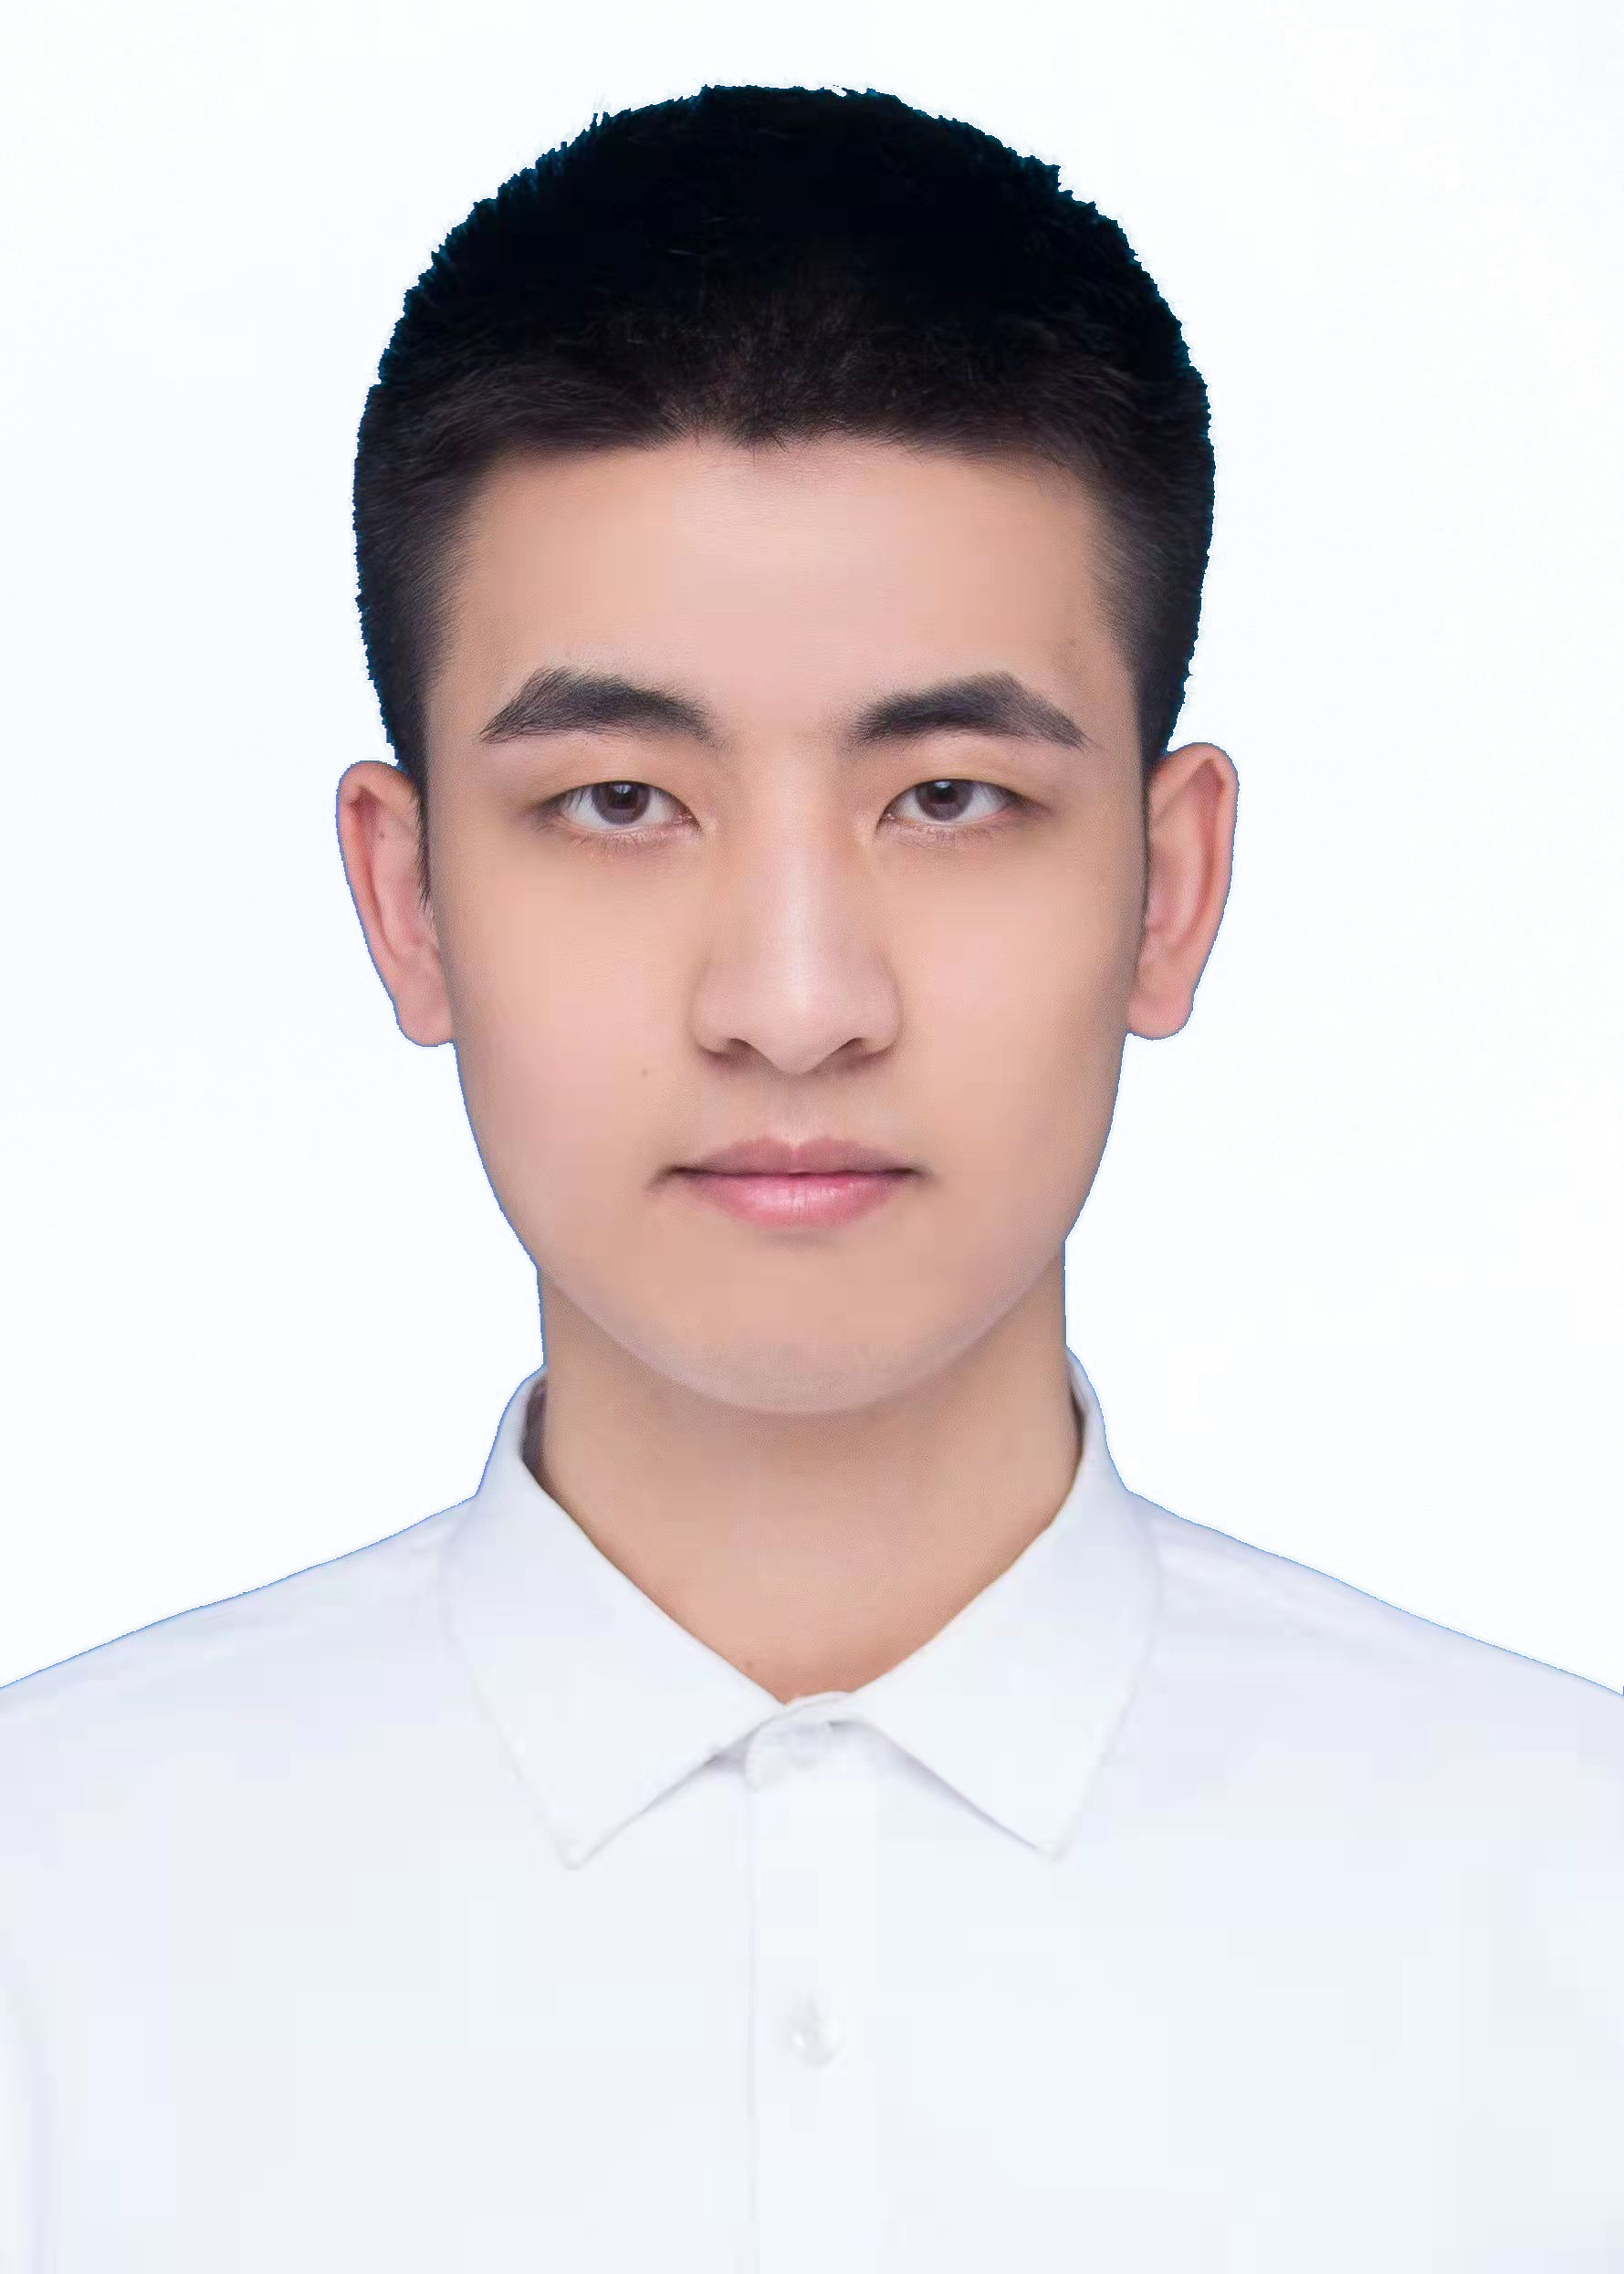
\includegraphics[width=0.88in]{lzj_avatar}} & \scshape{Zujing Liu} \\
%     & \email{zujing.liu@whu.edu.cn} \\
%     & \phone{(+86) 187-9005-5889} \\
%     & \homepage[liuxiaozhu.github.io]{https://liuxiaozhu01.github.io/} \\
%     & \github[github.com/liuxiaozhu01]{https://github.com/liuxiaozhu01} 
%   \end{tabu}
% }
% }

{
% change Large font here
\Large{
  \begin{tabularx}{\textwidth}{@{} c X r @{}}
   \multirow{4}{1in}[1.em]{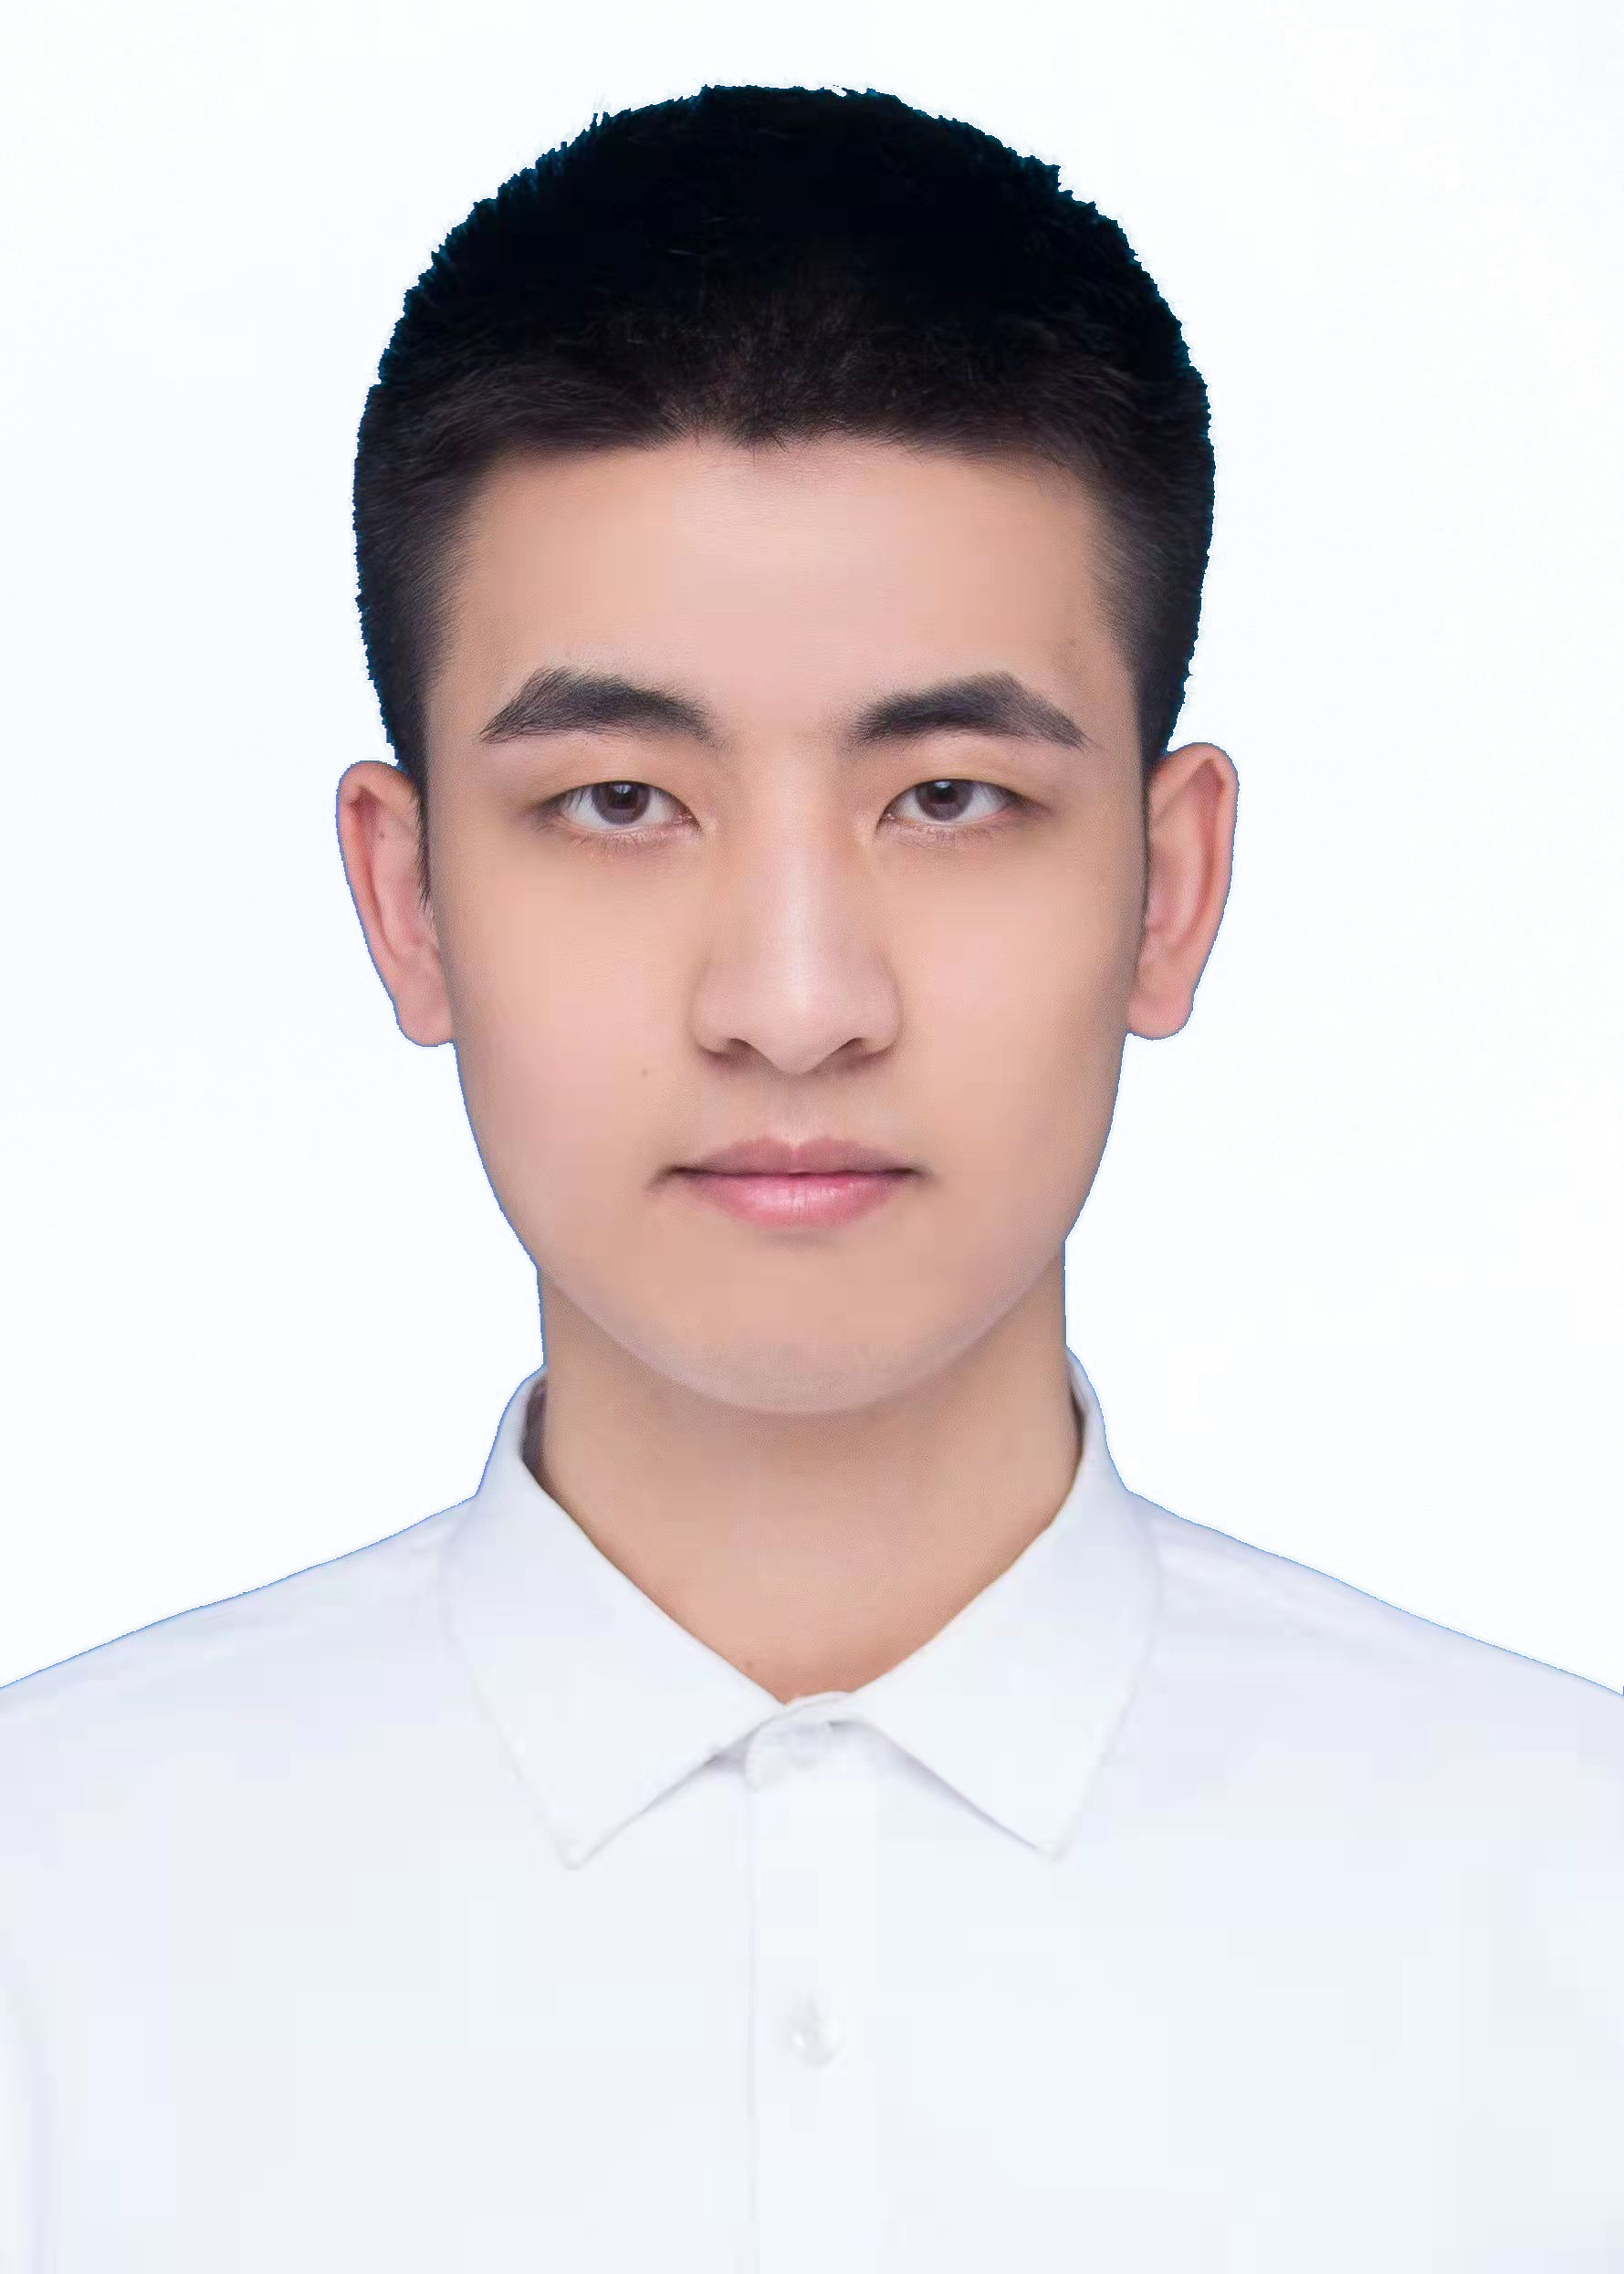
\includegraphics[width=0.88in]{lzj_avatar}} & \scshape{Zujing Liu (刘祖靖)} & \email{zujing.liu@whu.edu.cn} \\
    & Wuhan University & \phone{(+86) 187-9005-5889} \\
    & Computer Science & \homepage[liuxiaozhu.github.io]{https://liuxiaozhu01.github.io/} \\
    &                  & \github[github.com/liuxiaozhu01]{https://github.com/liuxiaozhu01} 
  \end{tabularx}
}
}

\section{\faGraduationCap\ Education}
\datedsubsection{\textbf{Wuhan University (WHU)}, Wuhan, China}{2023.09 -- Present}
\textit{Master student} in Computer Science (CS), advised by Prof. Gui-song Xia and Prof. Yuan Gao
\datedsubsection{\textbf{Wuhan University (WHU)}, Wuhan, China}{2019.09 -- 2023.07}
\textit{B.S.} in Computer Science (CS) with Honor Degree from Hongyi Honor College

\section{\faUsers\ Experience}
\datedsubsection{\textbf{Bypass Back-propagation: Optimization-based Structural Pruning for Large Language Models via Policy Gradient}}{ACL Under Review}
% \role{Summer Intern}{Manager: xxx}
% Brief introduction: xxx.
\begin{itemize}
  \item A novel optimization-based structural pruning method for LLM that optimizes directly for model loss.
  \item Learning pruning mask using Bernoulli distribution via policy gradient estimator to avoid back-propagation.
  \item Superior performance compared to existing techniques, with efficient computation on a single GPU.
\end{itemize}

% \datedsubsection{\textbf{xxx Projects}}{Jan. 2015 -- Present}
% \role{C, Python, Django, Linux}{Individual Projects, collaborated with xxx}
% Brief introduction: xxx
% \begin{itemize}
%   \item Implemented xxx feature
%   \item Optimized xxx 5\%
%   \item xxx
% \end{itemize}

% \datedsubsection{\textbf{\LaTeX\ résumé template}}{May. 2015 -- Present}
% \role{\LaTeX, Maintainer}{Individual Projects}
% An elegant \LaTeX\ résumé template, https://github.com/billryan/resume
% \begin{itemize}
%   \item Easy to be further customized or extended
%   \item Full support for unicode characters (e.g. CJK) with \XeLaTeX\
%   \item FontAwesome 4.5.0 support
% \end{itemize}

% Reference Test
%\datedsubsection{\textbf{Paper Title\cite{zaharia2012resilient}}}{May. 2015}
%An xxx optimized for xxx\cite{verma2015large}
%\begin{itemize}
%  \item main contribution
%\end{itemize}

% \section{\faCogs\ Skills}
% \begin{itemize}[parsep=0.5ex]
%   \item Programming Languages: C == Python > C++ > Java
%   \item Platform: Linux
%   \item Development: Web, xxx
% \end{itemize}

% \section{\faHeartO\ Honors and Awards}
% \datedline{\textit{\nth{1} Prize}, Award on xxx }{Jun. 2013}
% \datedline{Other awards}{2015}

\section{\faTrophy\ Honors and Awards}
\datedsubsection{Bachelor Stages}{2019 -- 2023}
\begin{itemize}[parsep=0.5ex]
  \item Second-Class Academic Scholarship of Wuhan University (2021)
  \item Outstanding Students of Wuhan University (2021)
  \item National Endeavor Scholarship
\end{itemize}

%% Reference
%\newpage
%\bibliographystyle{IEEETran}
%\bibliography{mycite}
\end{document}
